\chapter{Seguridad y ética}\label{ch:seguridad-y-etica}

La adopción de animales es un proceso que requiere de una gran responsabilidad por parte de los adoptantes. Por ello,
la seguridad de los datos es un tema importante a tener en cuenta en este proyecto para asegurar que los usuarios
se sientan cómodos y seguros a la hora de utilizar la aplicación. Para conseguirlo, se han tomado una serie de medidas
que se explicarán en este capítulo como la encriptación de datos, el registro de usuarios por medio de doble
factor de autenticación, la gestión de la información y los términos y condiciones de uso. \\

La ética también es otra consideración importante en el proyecto ya que es importante evitar que se fomente
la compra de animales, la cría irresponsable, el abandono de mascotas y la explotación animal. Las organizaciones
y asociaciones que se dedican a la adopción de animales tienen como objetivo principal el bienestar de los animales
y la concienciación de la sociedad. Por ello, es importante que la aplicación no se utilice para fines distintos
a los que se ha diseñado y que se cumplan los términos y condiciones de uso establecidos (ver sección~\ref{subsec:terminos-y-condiciones}).

\section{Seguridad}\label{sec:seguridad}

Como se ha mencionado, la \textbf{seguridad} de los datos en un proyecto de este tipo es crucial para que los usuarios no
comprometan su información personal. Por ello, se han tomado una serie de medidas para garantizar la seguridad
de los mismos tanto en la \textbf{API} como en la página web y en la base de datos.

\subsection{API}\label{subsec:api}

Para el desarrollo seguro de la API se han seguido las recomendaciones de seguridad de la documentación de \textit{FastAPI}
y se han implementado las siguientes medidas:

\begin{itemize}
    \item \textbf{Encriptación de datos}: se ha utilizado la librería \textit{pycryptodome} para encriptar las contraseñas de los
    usuarios y evitar que se puedan ver en texto plano. Para ello, se ha utilizado el algoritmo \textit{AES} (Advanced Encryption Standard) con una clave
    de 32 bytes y un vector de inicialización de 16 bytes. La clave y el vector de inicialización se han generado
    aleatoriamente y se han guardado en el fichero \textit{.env} para que no se puedan ver en el código fuente. Este algoritmo
    consiste en una serie de rondas de sustitución y permutación de bits que se repiten 10, 12 o 14 veces dependiendo
    del tamaño de la clave. El tamaño de la clave se mide en bits y puede ser de 128, 192 o 256 bits. Cuanto mayor sea
    el tamaño de la clave, más segura será la encriptación. En este caso, se ha utilizado una clave de 256 bits que
    es la más segura de las tres. Fuente:~\cite{aes}
        \begin{figure}[H]
            \centering
            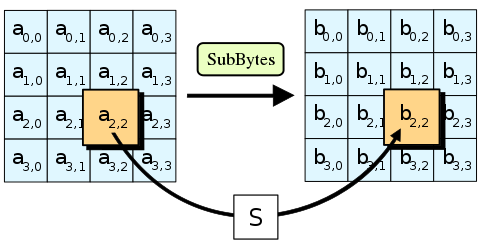
\includegraphics[width=0.8\textwidth]{imgs/aes.png}
            \caption{Encriptación de datos con AES. Fuente de imagen: \href{https://es.wikipedia.org/wiki/Advanced_Encryption_Standard}{Wikipedia}}
            \label{fig:encriptacion}
        \end{figure}
    \item \textbf{Autenticación y autorización}: se ha utilizado el protocolo estándar \textit{OAuth2} para la autenticación y autorización de usuarios.
    Este estándar permite que los usuarios autoricen a una aplicación a acceder a sus datos en otro servicio sin tener
    que compartir sus credenciales. Para ello, se ha utilizado la librería \textit{OAuth2} de \textit{FastAPI} que permite
    generar tokens de acceso y tokens de actualización. Los tokens de acceso se utilizan para acceder a los recursos
    protegidos y los tokens de actualización se utilizan para obtener nuevos tokens de acceso cuando estos han expirado.
    \item \textbf{Validaciones de datos}: se han utilizado las validaciones de datos de \textit{FastAPI} para asegurar que los datos
    que se envían a la \textbf{API} son correctos. Para ello, se han utilizado los tipos de datos de \textit{Pydantic} que permiten
    definir los tipos de datos de cada campo y las validaciones que deben cumplir. Por ejemplo, se ha definido que
    los números de teléfono deben tener el prefijo de España (+34) seguido de 9 dígitos y que los correos electrónicos deben tener el formato
    correcto. Además, se han definido los campos que son obligatorios y los que son opcionales para cada \textit{endpoint}.
    \item \textbf{Auditoría}: por medio de \textbf{Render} se ha podido monitorizar el uso de la \textbf{API} y comprobar que los usuarios
    no hacen un uso indebido de la misma. Se puede controlar el número de peticiones que se hacen a cada \textit{endpoint},
    la forma en la que se hacen las peticiones y el tiempo de respuesta de cada una de ellas. Además, se puede controlar
    el número de usuarios que se registran en la aplicación y el número de usuarios que se autentican en la misma.
    \item \textbf{Doble factor de autenticación}: para evitar que los usuarios puedan crear cuentas con datos falsos, se ha
    implementado un sistema de doble factor de autenticación. Gracias a los servicios de \textit{Firebase}, cada vez que
    un usuario u organización se registra en la aplicación, se le envía un correo electrónico con un enlace para verificar
    su cuenta. De esta forma, se evita que se puedan crear cuentas con datos falsos y se asegura que los usuarios
    que se registran en la aplicación son reales. Cuando se quiere restaurar la contraseña ocurre lo mismo, se envía
    un correo electrónico con un enlace para que el usuario pueda cambiar su contraseña.
    \item \textbf{Sistema seguro de contraseñas}: para evitar que las contraseñas de los usuarios sean vulnerables, se ha
    impuesto una serie de restricciones a la hora de crear una contraseña. Las contraseñas deben tener una longitud mínima
    de 8 caracteres y deben contener al menos una letra mayúscula, una letra minúscula, un número y un carácter especial
    \item \textbf{Vulnerabilidad en endpoints}: para evitar que un ataque de fuerza bruta pueda vulnerar la seguridad de la \textbf{API},
    los códigos de respuesta de cada \textit{endpoint} no dan información valiosa sobre el error que se ha producido. Por ejemplo,
    si se quisiera restaurar la contraseña de un usuario y se envía un correo electrónico que no está registrado en la
    aplicación, el código de respuesta sería 200 (OK) en lugar de 404 (Not Found). De esta forma, se evita que un atacante
    pueda saber si un correo electrónico está registrado en la aplicación o no.
\end{itemize}

Toda esta serie de medidas de seguridad permiten que la \textbf{API} sea en la medida de lo posible segura y que los usuarios
puedan hacer uso de ella sin tener que preocuparse por la seguridad de sus datos, lo cual garantiza la permanencia
de los mismos en el tiempo.

\subsection{Página web}\label{subsec:pagina-web}

Para la página web también se han tomado medidas de seguridad para garantizar la seguridad de los datos de las organizaciones.
En este caso, se ha utilizado el protocolo \textit{HTTPS} (Hyper Text Transfer Protocol Secure) que es la versión segura
del protocolo \textbf{\textit{HTTP}}. Este protocolo permite que los datos que se envían entre el servidor y el cliente estén encriptados
y que no puedan ser leídos por terceros. Para ello, se ha utilizado un certificado \textbf{\textit{TSL (Transport Layer Security)}} que
es un protocolo que permite la comunicación segura entre dos entidades. Es un archivo digital que se utiliza para verificar
la identidad de un sitio web o servidor y para encriptar la información que se envía entre el servidor y el cliente.
Cuando un usuario accede a un sitio web que utiliza \textbf{\textit{HTTPS}} (protocolo seguro basado en TLS), el navegador web
autentica el servidor web y luego utiliza la clave pública del servidor para encriptar la información que se envía al
servidor. El servidor web desencripta la información utilizando su clave privada y luego procesa la información. De esta
forma, se garantiza que los datos que se envían entre el servidor y el cliente están encriptados y que no pueden ser
leídos por terceros. \\

También por medio de \textbf{tokens} como \textbf{JWT} (JSON Web Token) se ha podido implementar un sistema de autenticación
y autorización seguro. Cuando un usuario se autentica en la aplicación, se le envía un token de acceso que contiene
información sobre el usuario y que tiene una duración de 15 minutos. Este token se utiliza para acceder a los recursos
protegidos de la aplicación. Cuando el token expira, se utiliza un token de actualización para obtener un nuevo token
de acceso. En la siguiente imagen se describe el proceso de login de un usuario en la aplicación:

\begin{figure}[H]
    \centering
    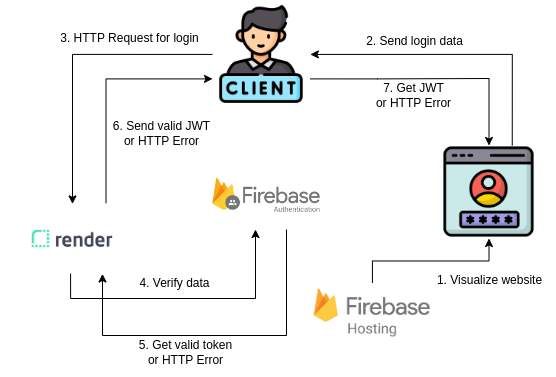
\includegraphics[width=0.8\textwidth]{imgs/login-diagrama.png}
    \caption{Proceso de login de un usuario en la aplicación}
    \label{fig:login}
\end{figure}

Como se puede observar en la imagen, cuando un usuario se autentica en la aplicación, se le envía un token de acceso
que contiene información sobre el usuario o un error en caso de que las credenciales sean incorrectas. Este token
se utiliza para acceder a los recursos protegidos de la aplicación. \\

Otra técnica que se ha utilizado para garantizar la seguridad de los datos de las organizaciones es la \textbf{protección \textit{CSRF}} (Cross-Site Request Forgery).
Esta técnica consiste en añadir un \textit{token} a cada formulario de la aplicación para evitar que un atacante pueda enviar
peticiones a la aplicación en nombre de un usuario. También por medio de los \textbf{encabezados \textit{CORS}} (Cross-Origin Resource Sharing) se ha
podido controlar el acceso a los recursos de la aplicación. Por ejemplo, se ha definido que solo se puede acceder a los
recursos de la aplicación desde la página web y no desde otras aplicaciones.

\newpage

\subsection{Base de datos}\label{subsec:base-de-datos}

La principal seguridad que se ha tomado en la base de datos ha sido la de crear reglas de seguridad de \textit{Firebase} tal
y como se ha explicado en la sección~\ref{subsec:firebase}. Estas reglas de seguridad permiten controlar el acceso a la
lectura y escritura de los datos de la base de datos. \\

\textbf{Firebase} utiliza los protocoles \textit{SSL/TLS} para cifrar las comunicaciones entre la aplicación y la base de datos. De
esta forma no se puede interceptar el tráfico de la aplicación y leer los datos que se envían a la base de datos. También
implementa protección frente a ataques de fuerza bruta, limitando el número de intentos de autenticación que se pueden hacer
en un periodo de tiempo por dirección IP. \\

Otra forma con la que \textbf{Firebase} protege los datos de la base de datos es con técnicas de prevención de inyección
de código malicioso en las consultas a la base de datos. Por ejemplo, si se intenta hacer una consulta a la base de datos
con una clave que no existe, se devuelve un error en lugar de devolver un resultado vacío. De esta forma, se evita que
un atacante pueda saber si una clave existe en la base de datos o no. \\

En resumen, gracias a todas las medidas de seguridad que implementa \textbf{Firebase}, se garantiza la seguridad de los
datos de las organizaciones y usuarios, se evita los posibles ataques contra la base de datos y hace que la aplicación
se convierta en una aplicación segura y fiable para todos los usuarios.

\section{Ética}\label{sec:etica}

Para abordar el tema de la ética en el desarrollo de la aplicación, se ha tenido en cuenta el código ético de la ACM (Association
for Computing Machinery)~\cite{acm-code-of-ethics}. Este código ético se basa en 7 principios generales que se deben tener en cuenta
a la hora de desarrollar un software. A continuación, se explica cómo se han aplicado estos principios en el desarrollo
de la aplicación web y \textbf{API}:

\begin{itemize}
    \item \textbf{Contribuir al bienestar y a la calidad de vida de los usuarios}: La aplicación se ha desarrollado con el
    objetivo de ayudar a las organizaciones a gestionar sus animales y a encontrarles un hogar. De esta forma, se contribuye
    al bienestar de los animales y a la calidad de vida de las personas que los adoptan.
    \item \textbf{Evitar daños a otros}: La aplicación no tiene ningún tipo de contenido que pueda dañar a los usuarios de
    la misma. Además, se han tomado medidas de seguridad para garantizar la seguridad de los datos de las organizaciones y
    de los usuarios.
    \item \textbf{Ser honesto y confiable}: La aplicación es honesta y confiable ya que no se ha ocultado ningún tipo de
    información a los usuarios y se ha desarrollado con el objetivo de ayudar a las organizaciones a gestionar sus animales
    y a encontrarles un hogar.
    \item \textbf{Ser justo y tomar medidas para no discriminar}: La aplicación no discrimina a ningún tipo de usuario
    siempre y cuando se cumplan las condiciones de uso de la misma.
    \item \textbf{Respetar el trabajo necesario para producir nuevas ideas, inventos, trabajos creativos y artefactos informáticos}:
    La aplicación respeta el trabajo necesario para producir nuevas ideas, inventos, trabajos creativos y artefactos informáticos
    ya que no se ha copiado ningún tipo de código de otras aplicaciones y se ha desarrollado desde cero.
    \item \textbf{Respetar la privacidad}: La aplicación respeta la privacidad de los usuarios ya que no se almacena ningún
    tipo de información personal de los usuarios y se ha implementado un sistema de autenticación y autorización seguro.
    \item \textbf{Respetar la confidencialidad}: La aplicación respeta la confidencialidad de los datos de las organizaciones
    y de los usuarios ya que se han tomado medidas de seguridad que se pueden ver en detalle en los apartados anteriores.
\end{itemize}

Para concluir con este apartado es interesante mencionar que a la hora de realizarse un registro en la aplicación web,
se necesitan aprobar los términos y condiciones de uso de la misma. En estos términos y condiciones se explica que la
aplicación no se hace responsable de los datos que se almacenan en la misma y que se pueden eliminar los datos de la
aplicación en cualquier momento. También se explica que la aplicación no se hace responsable de los daños que se puedan
ocasionar por el uso de la misma y que se pueden modificar los términos y condiciones en cualquier momento.

\subsection{Gestión de la información}\label{subsec:gestion-de-la-informacion}

En este apartado se explica cómo se ha gestionado la información de los usuarios y de las organizaciones. \\

En primer lugar, se ha tenido en cuenta la \textbf{Ley Orgánica de Protección de Datos}~\cite{ley-proteccion-datos} (LOPD) que
regula el tratamiento de los datos personales y las obligaciones que deben asumir los responsables de una web o una
aplicación web que almacene datos de carácter personal. \\

En esta ley se establece que los datos de carácter personal deben ser tratados de forma lícita, leal y transparente en
relación con el interesado y recogidos con fines determinados, explícitos y legítimos. También se establece que los datos
de carácter personal deben ser adecuados, pertinentes y limitados a lo necesario en relación con los fines para los que
son tratados. \\

Teniendo en cuenta esta ley y las diferentes medidas de seguridad que se han tomado en la aplicación, se puede afirmar
que se ha gestionado la información de los usuarios y de las organizaciones de forma correcta y que se ha cumplido con
la LOPD en todo momento durante el desarrollo de la aplicación web y \textbf{API}.

\subsection{Términos y condiciones}\label{subsec:terminos-y-condiciones}

Para realizar el registro en la aplicación web, se deben aceptar los términos y condiciones de uso de la misma. En estos
términos y condiciones es importante identificar los siguientes puntos:

\begin{itemize}
    \item \textbf{Responsabilidad}: La aplicación no se hace responsable de los datos que se almacenan en la misma y que
    se pueden eliminar los datos de la aplicación en cualquier momento.
    \item \textbf{Daños}: La aplicación no se hace responsable de los daños que se puedan ocasionar por el uso de la misma.
    \item \textbf{Modificación}: La aplicación se reserva el derecho de modificar los términos y condiciones en cualquier
    momento.
    \item \textbf{Aceptación}: La aceptación de los términos y condiciones es obligatoria para poder registrarse en la
    aplicación web.
    \item \textbf{Uso}: El uso de la aplicación web está limitado a las organizaciones que se dedican a la protección de
    animales y no a cualquier tipo de usuario que quiera registrarse en la aplicación.
    \item \textbf{Datos personales}: La aplicación no almacena ningún tipo de información personal de los usuarios.
    \item \textbf{Actualización y revisión}: La aplicación se reserva el derecho de actualizar y revisar los términos y
    condiciones en cualquier momento.
\end{itemize}

En la siguiente imagen vemos como en el registro se añade un checkbox para aceptar los términos y condiciones de uso de
la aplicación web: \\

\begin{figure}[H]
    \centering
    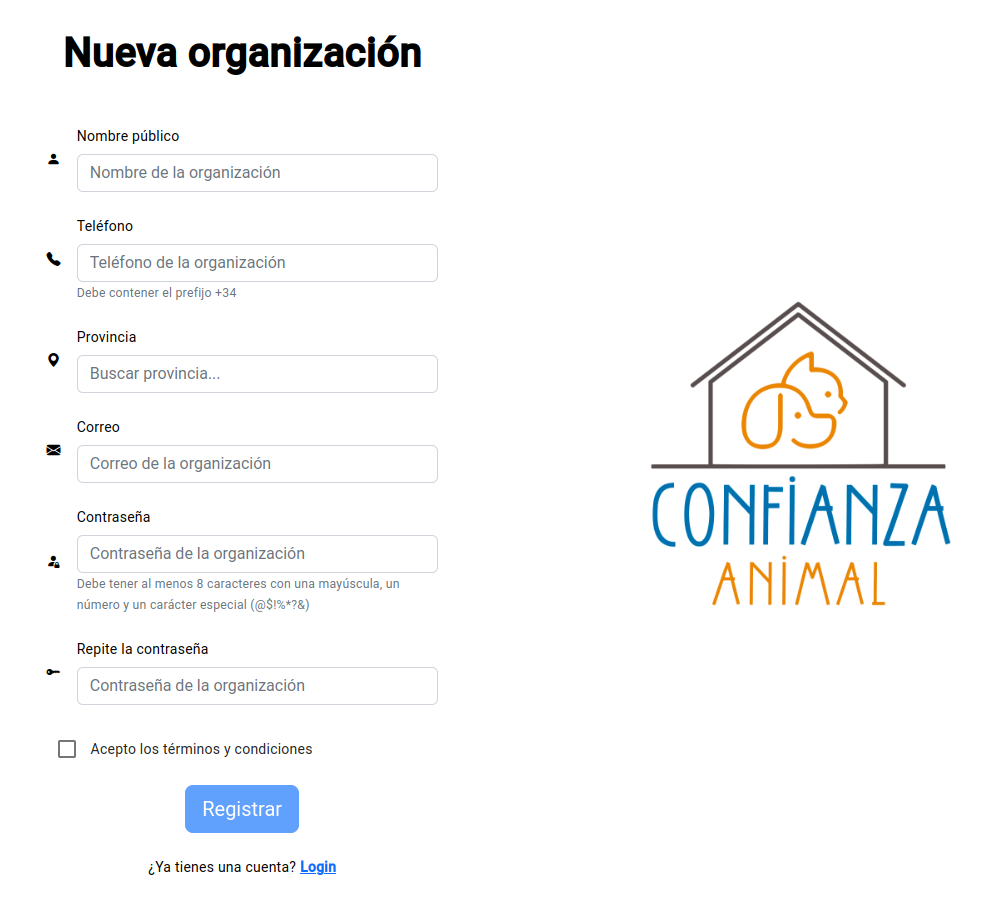
\includegraphics[width=0.9\textwidth]{imgs/registro.png}
    \caption{Registro de organizaciones en aplicación web}
    \label{fig:terminos-y-condiciones}
\end{figure}